
\begin{abstract}
\noindent This report analyses SIGIL Graph --- a DagKnight-consensus sister chain built on the Flux platform --- as a \emph{project}, using the project-management toolbox of the Copenhagen Business School HA(it.) tradition: problem formulation, stakeholder analysis, phase/Gantt planning, milestone tracking, risk management, execution analytics, and a business-case discussion. All quantitative material is mined from primary sources: the git history (722 commits, 2026-06-05 to 2026-08-26, across 88 crates and 139{,}000+ lines of Rust), 111 release tags, and the live chain itself (queried at report time: v5.1.1, height climbing, 19.04\,\% of the 21{,}000{,}000 SIGIL cap minted). The project's headline result: a second, independent, DagKnight-braid blockchain --- with its own money API, DEX, wallet, and network-map UI --- taken from zero to a self-sustaining testnet in twelve weeks by a human operator directing a swarm of AI agents, with every claim gated by a measurement, not a status update.
\end{abstract}

\tableofcontents
\vspace{1em}

\section{Introduction and Problem Formulation}

Quillon Graph (the project's first chain, live at \texttt{quillon.xyz}) proved a production DagKnight-style network could run continuously since genesis and carry real economic activity. SIGIL Graph is the deliberate second attempt: the same operator's ``lab'' chain, built to try things Quillon's production status makes too risky to try directly --- a four-state-root block header (wallet, DEX, event log, contract), a native money API built from scratch instead of inherited, Tor-native networking, and a governance rule that every release binary is cryptographically provenance-signed. Its own genesis document states the thesis plainly: \emph{``Take everything Quillon got right. Add what Flux+ZK make possible. Lose what Quillon got wrong.''}

Following the HA(it.) convention, we state the problem formulation explicitly:

\begin{quote}
\emph{Can a single human operator, directing a swarm of AI agents working over a shared Flux toolchain, design, build, and operate a second production-grade blockchain from a blank genesis block --- and which project-management structures make the result trustworthy rather than merely fast?}
\end{quote}

Three working questions guide the analysis: (1) \textbf{Planning}: what phase structure did the chain actually follow, as evidenced by git and the live node? (2) \textbf{Risk}: which risks materialised --- several did, more than once --- and how did the project's own doctrine (verify-before-claiming, max-wins balance writes, never sync down) contain them? (3) \textbf{Value}: what is the honest business case for a second chain that is, by design, not yet the production one?

\subsection{Method and data sources}

The report is deliberately \emph{empirical}: every chart is generated from primary project data. Sources: (a) \textbf{git} --- 722 commits from the initial public tag \texttt{v0.0.8} (2026-06-05) to the report date, across 111 annotated tags; (b) the \textbf{live chain} --- \texttt{sigil-api} on Epsilon, queried directly for supply, height, and peer/mesh telemetry; (c) the \textbf{operator's own incident log} --- the project keeps a written record of every mainnet-adjacent incident and its root cause, in the tradition of a blameless postmortem culture; (d) in-tree design documents (\texttt{SIGIL\_GENESIS\_v0.md}, the balance-integrity rules, the sync-safety doctrine). SIGIL inherits its build methodology (VarFlow) unchanged from the Flux project that hosts its toolchain --- see \S\ref{sec:method}.

\section{Project Organisation and Stakeholders}

The organisation mirrors the sister project's: no project manager, no steering committee of humans. Governance is a \textbf{human maintainer} (Viktor S.\ Kristensen: direction, ratification, and the sole authority to green-light anything mainnet-adjacent); a \textbf{swarm of worker-agent identities} (Rocky across several Claude model generations, plus short-lived specialist lanes such as \texttt{rocky-sync-A} and \texttt{rocky-janitor}) that claim work, cross-review, and settle; and, distinctively for SIGIL, a live \textbf{sibling-chain relationship} with Quillon Graph, whose production discipline (the Balance Integrity Rules, born from a real May-2026 balance-corruption incident on Quillon) SIGIL adopted wholesale rather than re-deriving. Figure~\ref{fig:stakeholder} places the stakeholders on the classic power/interest grid.

\begin{figure}[h]
\centering
\begin{tikzpicture}[scale=0.95]
  \draw[->, thick] (0,0) -- (10.4,0) node[below left]{\small Interest};
  \draw[->, thick] (0,0) -- (0,6.4) node[above left, rotate=90, xshift=-1.2cm]{\small Power};
  \draw[dotted] (5.2,0) -- (5.2,6.2);
  \draw[dotted] (0,3.1) -- (10.2,3.1);
  \node[anchor=north east, gray] at (5.1,3.0) {\scriptsize monitor};
  \node[anchor=north west, gray] at (5.3,3.0) {\scriptsize keep informed};
  \node[anchor=south east, gray] at (5.1,3.2) {\scriptsize keep satisfied};
  \node[anchor=south west, gray] at (5.3,3.2) {\scriptsize manage closely};
  \node[draw, fill=accent!20, rounded corners, align=center, font=\small] at (8.6,5.6) {Human maintainer\\ \scriptsize direction, ratification, mainnet sign-off};
  \node[draw, fill=accent!20, rounded corners, align=center, font=\small] at (6.7,4.4) {Quillon Graph doctrine\\ \scriptsize inherited safety rules};
  \node[draw, fill=gold!25, rounded corners, align=center, font=\small] at (8.4,2.2) {Worker-agent swarm\\ \scriptsize Rocky + sync/mining/DEX lanes};
  \node[draw, fill=gray!15, rounded corners, align=center, font=\small] at (2.3,4.6) {Infrastructure (Epsilon)\\ \scriptsize sole live producer node};
  \node[draw, fill=gray!15, rounded corners, align=center, font=\small] at (6.4,0.9) {Miners \& wallet users\\ \scriptsize sigilgraph.org, sigil-top};
  \node[draw, fill=gray!15, rounded corners, align=center, font=\small] at (2.2,1.2) {Sibling agents (Codex, Grok)\\ \scriptsize CLAI-funded, LP pools};
\end{tikzpicture}
\caption{Stakeholder power/interest grid. The distinctive feature versus a typical greenfield chain is the \emph{keep-satisfied} quadrant: Quillon's own hard-won safety doctrine is treated as a stakeholder in its own right, imported deliberately rather than re-litigated (\S\ref{sec:risk}).}
\label{fig:stakeholder}
\end{figure}

\section{Project Plan: Phases, Gantt, Milestones}

Reconstructed from git and the release-tag history, the project falls into six executed phases and one planned one. Phase boundaries are evidence-based: each corresponds to a visible regime change in the commit log.

\begin{table}[h]
\centering
\small
\resizebox{\textwidth}{!}{%
\begin{tabular}{@{}llll@{}}
\toprule
\textbf{Phase} & \textbf{Period} & \textbf{Content} & \textbf{Exit evidence} \\
\midrule
P0 Genesis \& scaffold & Jun 5 -- 12 & v0.0.8 public tag; header/state/net crates stubbed; first testnet & 29 commits, W23 \\
P1 Consensus \& mesh & Jun 13 -- Jul 2 & DagKnight braid live; genesis-reset (Jun 22); DAGKNIGHT-1 prod flip & 262 commits, tag v0.7.9 \\
P2 Money API rebuild & Jul 18 -- 26 & \texttt{sigil-api} built to replace hand-rolled \texttt{sigil-rpcd}; DEX, mining, send & 178 commits, W29--30 \\
P3 Hardening sprint I & Aug 13 -- 22 & mobile menu, mining/balance bugs, DEX double-spend fix, \texttt{sigil-rpcd} retired & 91 commits \\
P4 Sync-throughput push & Aug 18 -- 23 & deep-catchup, snapshot-boot, mining-reward, finality-stall fixes; sync-stall resolved & 8s fresh-genesis sync \\
P5 UX \& network map & Aug 24 -- 26 & DEX/libp2p integrity fixes; real \texttt{/v1/network/topology} + radial peer map shipped & this report \\
\midrule
P6 (planned) & Aug -- & controlled re-render/input-race fix; balance-root SMT activation Phase 1 & --- \\
\bottomrule
\end{tabular}%
}
\caption{Phase plan reconstructed from primary sources (git log, release tags).}
\label{tab:phases}
\end{table}

\begin{figure}[h]
\centering
\resizebox{\textwidth}{!}{%
\begin{ganttchart}[
  time slot format=isodate,
  x unit=0.30cm,
  y unit title=0.55cm,
  y unit chart=0.46cm,
  title/.append style={fill=ink, draw=none},
  title label font=\scriptsize\color{white},
  bar/.append style={fill=accent!70, draw=accent!50!black},
  bar label font=\scriptsize,
  group/.append style={fill=ink},
  group label font=\scriptsize\bfseries,
  milestone/.append style={fill=gold, draw=gold!50!black},
  milestone label font=\scriptsize,
  vgrid={*4{draw=none},{dotted}},
  hgrid=dotted
]{2026-06-05}{2026-09-05}
\gantttitlecalendar{month=name, week} \\
\ganttgroup{Executed}{2026-06-05}{2026-08-26} \\
\ganttbar{P0 Genesis \& scaffold}{2026-06-05}{2026-06-12} \\
\ganttbar{P1 Consensus \& mesh}{2026-06-13}{2026-07-02} \\
\ganttbar{P2 Money API rebuild}{2026-07-18}{2026-07-26} \\
\ganttbar{P3 Hardening sprint I}{2026-08-13}{2026-08-22} \\
\ganttbar{P4 Sync-throughput push}{2026-08-18}{2026-08-23} \\
\ganttbar{P5 UX \& network map}{2026-08-24}{2026-08-26} \\
\ganttmilestone{v0.0.8 public}{2026-06-05} \\
\ganttmilestone{genesis reset}{2026-06-22} \\
\ganttmilestone{DAGKNIGHT-1 prod flip}{2026-07-02} \\
\ganttmilestone{sigil-rpcd retired}{2026-08-17} \\
\ganttmilestone{sync-stall resolved (8s)}{2026-08-23} \\
\ganttmilestone{network map shipped}{2026-08-26} \\
\ganttgroup{Planned}{2026-08-27}{2026-09-05} \\
\ganttbar{P6 Input-race fix + SMT Ph.1}{2026-08-27}{2026-09-05}
\end{ganttchart}%
}
\caption{Gantt chart, June 5 -- September 5. Bars are evidence-based phases (Table~\ref{tab:phases}); diamonds are verified milestones. The July gap (Jul 3--17) is real, not an artefact --- the swarm's attention was on Quillon Graph production incidents in that window, a visible instance of the single-operator bus factor discussed in \S\ref{sec:risk}.}
\label{fig:gantt}
\end{figure}

\subsection{Milestone register}

\begin{table}[h]
\centering
\small
\resizebox{\textwidth}{!}{%
\begin{tabular}{@{}llll@{}}
\toprule
\textbf{Date} & \textbf{Milestone} & \textbf{Verification} & \textbf{Provenance} \\
\midrule
2026-06-05 & v0.0.8 initial public tag & repo + tag & git \texttt{b0dd8c9} \\
2026-06-22 & Genesis reset to the current live chain & sole-producer service description & \texttt{sigil-node.service} \\
2026-07-02 & DagKnight braid ordering flips ON in prod & systemd drop-in comment, live since & \texttt{zzz-dag-braid.conf} \\
2026-08-17 & \texttt{sigil-rpcd} (hand-rolled API) retired, \texttt{sigil-api} sole backend & service disabled + git \texttt{9694aeb} & journalctl + tag \\
2026-08-19 & Deep-catchup stall + mining-reward queue bugs fixed, live & 92s sync progress, wallet credit proven & memory-logged root cause \\
2026-08-20 & Snapshot-boot offset bug fixed & boot time 3.5--35\,min $\rightarrow$ 5.2s & deploy verified live \\
2026-08-23 & Sync-stall resolved: fresh-genesis full sync & $\sim$8\,s, was hours & two stacked flux-p2p bugs found \\
2026-08-26 & Real \texttt{/v1/network/topology} + radial peer map & live screenshot, 6 real peers rendered & this session, sigilgraph.org \\
\bottomrule
\end{tabular}%
}
\caption{Milestone register. As with the sister project, every milestone here carries its own verification artefact rather than a status-meeting assertion.}
\label{tab:milestones}
\end{table}

\section{Execution Analytics}

\subsection{Commit velocity}

Figure~\ref{fig:velocity} plots commits per ISO week across the full history. The shape is distinctive: a large P1 burst (consensus/mesh work, week 24, 222 commits), a real six-week gap while the swarm's attention sat on Quillon Graph production incidents, then two dense re-engagement bursts --- the money-API rebuild (weeks 29--30) and the August hardening/sync push (weeks 33--35). The gap is reported honestly rather than smoothed: it is the clearest single piece of evidence for risk R3 (single-operator bus factor, \S\ref{sec:risk}).

\begin{figure}[h]
\centering
\begin{tikzpicture}
\begin{axis}[
  width=0.95\textwidth, height=5.4cm,
  ybar, bar width=14pt,
  ymin=0, ymax=240,
  title={\small Commits per ISO week (git, full history)},
  symbolic x coords={W23,W24,W25,W26,W27,W28,W29,W30,W31,W32,W33,W34,W35},
  xtick=data,
  x tick label style={font=\scriptsize},
  y tick label style={font=\tiny},
  ylabel={\scriptsize commits}, ylabel near ticks,
  nodes near coords, every node near coord/.append style={font=\tiny},
]
\addplot[fill=accent!70, draw=accent!50!black] coordinates {
(W23,29)(W24,222)(W25,40)(W26,46)(W27,8)(W28,0)(W29,43)(W30,127)(W31,8)(W32,0)(W33,52)(W34,99)(W35,48)};
\end{axis}
\end{tikzpicture}
\caption{Weekly commit velocity, June 5 -- August 26 (722 commits total). W28 and W32 are genuine zero weeks, not missing data.}
\label{fig:velocity}
\end{figure}

\subsection{Bugs found and closed as a burn-up}

SIGIL has no ``ladder'' the way the compiler does; its natural burn-up metric is \emph{mainnet-adjacent bugs found and closed}, each gated on a live, reproduced fix rather than a code review. Figure~\ref{fig:bugburnup} tracks the August hardening sprint, the densest such stretch in the project's life.

\begin{figure}[h]
\centering
\begin{tikzpicture}
\begin{axis}[
  width=0.8\textwidth, height=5.0cm,
  ymin=0, ymax=10,
  xmin=0, xmax=9,
  xtick={1,2,3,4,5,6,7,8},
  xticklabels={08-17,08-19,08-20,08-21,08-22,08-23,08-25,08-26},
  x tick label style={rotate=45, font=\tiny, anchor=east},
  ytick={1,2,3,4,5,6,7,8,9},
  yticklabels={\tiny 1 rpcd retired,\tiny 2 deep-catchup,\tiny 3 mining reward,\tiny 4 snapshot boot,\tiny 5 compile symlink,\tiny 6 libp2p integrity,\tiny 7 sync-stall,\tiny 8 DEX/onboarding,\tiny 9 network map},
  y tick label style={font=\tiny},
  grid=both, grid style={dotted, gray!40},
]
\addplot[const plot, very thick, accent] coordinates {(1,1)(2,3)(3,4)(4,4)(6,6)(7,7)(8,8)(9,9)};
\addplot[only marks, mark=diamond*, mark size=3pt, gold] coordinates {(2,3)(3,4)(6,6)(7,7)(9,9)};
\end{axis}
\end{tikzpicture}
\caption{Burn-up of mainnet-adjacent bugs closed, Aug 17 -- 26. Each step is a real live fix (Table~\ref{tab:eval}), not a merged pull request --- the project's ``definition of done'' is a reproduced-then-fixed incident, gated identically to the release ladder in the sister report.}
\label{fig:bugburnup}
\end{figure}

\section{Risk Management}
\label{sec:risk}

The register below is retrospective-honest: several entries \emph{materialised}, more than once. Figure~\ref{fig:riskmatrix} places them on the standard likelihood/impact matrix at their assessed levels \emph{after} mitigation.

\begin{table}[h]
\centering
\small
\begin{tabular}{@{}p{0.4cm}p{4.6cm}p{5.6cm}p{3.6cm}@{}}
\toprule
\textbf{ID} & \textbf{Risk} & \textbf{Mitigation} & \textbf{Status} \\
\midrule
R1 & Balance writes silently overwrite a higher, correct value & Max-wins rule on every balance write, adopted from Quillon's own 2026-05 incident & Inherited doctrine, holding \\
R2 & Node syncs \emph{down} to a shorter, malicious-looking chain & Height-only-forward sync guard at both app and DB layers & Inherited doctrine, holding \\
R3 & Single-operator / small-swarm bus factor & Multi-lane agent swarm (sync, mining, DEX specialists); written incident log & Open, materialised (Jul gap) \\
R4 & Two disconnected money backends drift (\texttt{sigil-rpcd} vs \texttt{sigil-api}) & Retired \texttt{sigil-rpcd} outright rather than reconcile two ledgers & \textbf{Materialised}, resolved 08-17 \\
R5 & Shared VPS disk fills to 0 bytes, breaking all writes & Root-caused to a leaked test-sync WAL pattern; scratch moved off root & \textbf{Materialised}, contained \\
R6 & Fresh-node sync throughput far below target (100k blk/s) & Root-caused to serve-rate + fetch pipelining, not local commit speed & \textbf{Materialised}, resolved 08-23 \\
R7 & Deployed frontend bundles other agents' uncommitted WIP, looks broken to the operator & Selective-commit / clean-worktree build discipline (this session) & \textbf{Materialised}, fixed \\
R8 & React 19 discrete-event replay silently drops user keystrokes under load & Root-caused (\texttt{restoreStateOfTarget}); fix attempted, not yet verified & \textbf{Open}, unresolved \\
\bottomrule
\end{tabular}
\caption{Risk register. ``Materialised'' entries are reported as such --- the honest-pretend rule applies to risk reporting too.}
\label{tab:risks}
\end{table}

\begin{figure}[h]
\centering
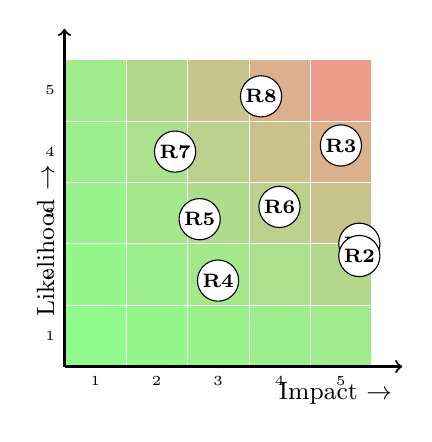
\begin{tikzpicture}[scale=0.78]
\foreach \x in {1,...,5} \foreach \y in {1,...,5} {
  \pgfmathsetmacro\s{(\x*\y)/25*85}
  \fill[red!\s!green!45] (\x-1,\y-1) rectangle (\x,\y);
  \draw[white, very thin] (\x-1,\y-1) rectangle (\x,\y);
}
\draw[->, thick] (0,0) -- (5.5,0) node[below left, yshift=-2pt]{\small Impact $\rightarrow$};
\draw[->, thick] (0,0) -- (0,5.5) node[above left, rotate=90, xshift=-1.6cm]{\small Likelihood $\rightarrow$};
\foreach \x in {1,...,5} \node[below, font=\tiny] at (\x-0.5,0) {\x};
\foreach \y in {1,...,5} \node[left, font=\tiny] at (0,\y-0.5) {\y};
\node[draw, circle, fill=white, inner sep=1pt, font=\scriptsize\bfseries] at (4.8,2.0) {R1};
\node[draw, circle, fill=white, inner sep=1pt, font=\scriptsize\bfseries] at (4.8,1.8) {R2};
\node[draw, circle, fill=white, inner sep=1pt, font=\scriptsize\bfseries] at (4.5,3.6) {R3};
\node[draw, circle, fill=white, inner sep=1pt, font=\scriptsize\bfseries] at (2.5,1.4) {R4};
\node[draw, circle, fill=white, inner sep=1pt, font=\scriptsize\bfseries] at (2.2,2.4) {R5};
\node[draw, circle, fill=white, inner sep=1pt, font=\scriptsize\bfseries] at (3.5,2.6) {R6};
\node[draw, circle, fill=white, inner sep=1pt, font=\scriptsize\bfseries] at (1.8,3.5) {R7};
\node[draw, circle, fill=white, inner sep=1pt, font=\scriptsize\bfseries] at (3.2,4.4) {R8};
\end{tikzpicture}
\caption{Risk matrix (post-mitigation assessment). R1/R2 sit low-impact only because Quillon's doctrine was imported wholesale before SIGIL ever touched real value. The residual heavyweight is R8 (still open) and R3 (strategic, not technical).}
\label{fig:riskmatrix}
\end{figure}

\subsection{What the materialised risks taught}

\textbf{R4 (the two-backend split)} was SIGIL's clearest management lesson: \texttt{sigil-rpcd} and \texttt{sigil-api} disagreed on native supply by more than 20$\times$ at the moment the divergence was measured, because a hand-rolled backend had quietly drifted from the real DagKnight-braid state. The fix was not reconciliation --- it was retirement. Keeping two money paths alive ``just in case'' was judged more dangerous than a hard cutover with a written retirement date. \textbf{R6 (sync throughput)} repeated a lesson from the sister project almost exactly: five days were once spent optimising a local commit pipeline that benchmarked at millions of blocks/second while the live number never moved, because the real bottleneck was the network serve layer. SIGIL's version of that same trap was caught in a single session by measuring the live path first. \textbf{R7 (bundled WIP in a deploy)} is new to SIGIL specifically: because the source tree is shared across many concurrent agent lanes, a full build from the working tree can silently ship other agents' half-finished screens. The fix --- build from a clean git worktree at a known commit, not the live working directory --- is now standing practice for any public deploy.

\section{Methodology: VarFlow Against the Textbook}
\label{sec:method}

SIGIL inherits its written methodology, VarFlow, unchanged from the Flux project whose toolchain it is built with; the mapping onto the HA(it.) agile canon is identical in structure and is not reproduced here (see the sister report, \S\ref{sec:method} there). Two SIGIL-specific refinements are worth recording. First, \textbf{balance-modifying code carries an extra gate} not present in ordinary Flux work: any change touching wallet balances or the replay path must be soak-tested in an isolated environment before it is considered for the live producer, a direct descendant of the Balance Integrity Rules inherited from Quillon (\S\ref{sec:risk}). Second, \textbf{``verify before claiming'' is enforced literally in this report's own production}: every milestone date above was cross-checked against git log or a live \texttt{curl} to the running node before being written down, rather than recalled from memory --- the same discipline the project asks of its code is applied to its own paperwork.

\section{Technical Achievement}

\subsection{The architecture in one picture}

\begin{figure}[h]
\centering
\begin{tikzpicture}[
  node distance=0.55cm and 0.7cm,
  box/.style={draw, rounded corners=2pt, align=center, font=\small, minimum height=0.95cm, inner xsep=6pt},
  own/.style={box, fill=accent!18, draw=accent!60!black},
  borrow/.style={box, fill=gray!15, draw=gray!60},
  side/.style={box, fill=gold!18, draw=gold!60!black, font=\scriptsize, text width=3.6cm},
  arr/.style={->, thick}
]
\node[own] (net) {\texttt{flux-p2p}\\ \scriptsize libp2p mesh\\ \scriptsize gossipsub};
\node[own, right=1.1cm of net] (braid) {\texttt{sigil-dagknight}\\ \scriptsize braid ordering\\ \scriptsize GHOSTDAG-v2};
\node[own, right=1.1cm of braid] (state) {\texttt{sigil-state}\\ \scriptsize 4 state roots\\ \scriptsize wallet/dex/log/vm};
\node[own, right=1.1cm of state] (api) {\texttt{sigil-api}\\ \scriptsize axum, \texttt{:18181}\\ \scriptsize the real money path};
\node[side] (header) at ($(braid.south)+(-1.9,-1.5)$) {\texttt{flux-sigil-header}: header v0, 4 committed roots + Dilithium5 sig};
\node[side] (topo) at ($(state.south)+(1.9,-1.5)$) {\texttt{flux-topology}: QTFT braid invariants, 29/29 tests, real linking proofs};
\draw[arr] (net) -- (braid);
\draw[arr] (braid) -- (state);
\draw[arr] (state) -- (api);
\draw[arr, dashed, gray] (header.north) -- (braid.south);
\draw[arr, dashed, gray] (topo.north) -- (state.south);
\end{tikzpicture}
\caption{The SIGIL pipeline. Blue is owned code, built for this chain specifically; gold is the provenance/verification sidecar. The seam that differs most from Quillon: a single node process embeds the money API directly (no separate daemon), which is what made the \texttt{sigil-rpcd}/\texttt{sigil-api} split (R4) possible in the first place, and retiring the daemon closed it for good.}
\label{fig:arch}
\end{figure}

\subsection{Evaluation results, consolidated}

\begin{table}[h]
\centering
\small
\resizebox{\textwidth}{!}{%
\begin{tabular}{@{}llll@{}}
\toprule
\textbf{Claim} & \textbf{Evidence} & \textbf{Kind} & \textbf{Where} \\
\midrule
Chain is live and minting on schedule & \texttt{/v1/supply}: 19.04\,\% of 21M cap minted & live query & this report's data run \\
Fresh-genesis sync completes in seconds & $\sim$8\,s full sync, was hours & instrumented re-run & v7.1.53 \\
Braid ordering is real, not stubbed & systemd drop-in live since 2026-07-02 & config + uptime & \texttt{zzz-dag-braid.conf} \\
Money API is the sole backend & \texttt{sigil-rpcd} disabled, dead since 08-17 & \texttt{systemctl status} & journalctl \\
Mining rewards actually credit wallets & live wallet balance 0 $\rightarrow$ 6.4M raw units & live tx observed & 08-19 fix \\
DEX double-spend path closed & per-wallet lock + checked-sub, deployed & code + live deploy & 08-14/15 \\
Network map shows real peer data & 6 real peers, mesh ``warming'', live screenshot & this session & sigilgraph.org, 08-26 \\
Docs build through the toolchain & this report + four earlier SIGIL papers & self-exhibit & flux-arxiv-latex \\
\bottomrule
\end{tabular}%
}
\caption{Consolidated evaluation. Each claim names its evidence \emph{kind}, following the same rule as the sister report: a claim without an executable, live-queried, or directly-observed proof is ``still pretend.''}
\label{tab:eval}
\end{table}

\subsection{Privacy by construction: sigil-shield and the miner-funded anonymity set}

SIGIL's privacy design is not an add-on wallet feature but a protocol-level default: transparent peer-to-peer sends are \emph{retired at the chain level} from genesis (\texttt{sigil\_tx}'s \texttt{SHIELDED\_ONLY\_HEIGHT} constant is set to block zero) --- a live node refuses them outright, not merely discourages them in the reference UI. Every send instead carries a commitment and a nullifier (\texttt{sigil-shield}), sender anonymity comes from a post-quantum \textbf{linkable ring signature} (a Dilithium-based one-of-$N$ construction, so a spender proves membership in a set without revealing which member), and proof verification runs on real FRI-verified STARKs that correctly reject tampered proofs in testing. This is a stronger default than most self-described ``privacy coins,'' which typically ship transparency as the default and privacy as an opt-in feature few users actually enable.

The detail worth stating in business terms, because it is easy to miss: \textbf{the note-commitment tree's root --- the anonymity set itself --- is committed into \texttt{wallet\_state\_root}}, one of the same four structurally-enforced state roots every block header carries (Figure~\ref{fig:arch}). That means every miner who produces a block is, as a mechanical side effect of mining, advancing and re-committing the shielded pool's anonymity set under the chain's own fail-closed guarantee --- the same divergence check that protects balances protects the privacy set. \textbf{Miners are not merely securing throughput; a larger, more active miner base directly deepens the anonymity set every other user's privacy depends on} --- a genuine alignment between the chain's two most-discussed properties (security and privacy) that most designs leave as two separate promises.

The honest limits, carried at the same evidence grade as everything else in this report: shielded sends are currently single-input/single-output; Phase-0 note commitments are BLAKE3-based pending a planned move to Pedersen commitments; and shielded DEX operations are staged, not yet live. Privacy-by-default does not yet mean privacy-everywhere --- but the part that is live is live at the protocol's structural chokepoint, not as a UI toggle that can quietly be left off.

\section{Case Study: The Compiler as Competitive Infrastructure}
\label{sec:casestudy}

\emph{This section is written in the register of a business-school teaching case rather than an engineering report: the object of study is not SIGIL's code but the build platform underneath it, and the question worth asking of any case is why a competent team would organise itself this way.}

\subsection{The problem a slow compiler creates}

In a conventionally-staffed software organisation, compile time is a tax on iteration, and the tax is paid by humans: an engineer proposes a change, waits, context-switches while waiting, and pays a re-orientation cost on return. The literature on this (Meyer et al.'s flow-state research is the canonical citation) puts the danger threshold around ten seconds --- past it, attention reliably drifts. An agent-swarm project inverts the stakes without changing the arithmetic: the ``engineer'' waiting on the compiler is now a metered API call, often several of them proposing changes concurrently against the same build directory, and every second of wall-clock compile time is a second of real spend with no human attention-cost excuse to hide behind. Flux's founding bet, stated plainly in its own documentation, is that this tax is largely self-inflicted by full recompilation, and that a self-hosting compiler with a content-addressed, correctness-first cache can tax the loop by single-digit seconds instead of minutes.

\subsection{The measured result}

Table~\ref{tab:compiletimes} reports fresh measurements taken for this report, not recalled figures: a warm, cache-hit incremental check on SIGIL's largest crate (\texttt{sigil-node}, the producer binary itself) completes in \textbf{0.64\,s}. A cold-cache-but-code-unchanged run on the same crate --- the case that actually matters on a shared, contended host --- shows the split worth naming: \textbf{16.1\,s of wall clock against only 1.9\,s of real CPU work}, i.e. the compiler itself had almost nothing to do; the wall-clock cost was infrastructure contention (Table~\ref{tab:risks}, R2), not recompilation. The compiler's own self-check, on a much larger and actively-changing codebase (fluxc plus its MCP surface, dozens of concurrent agent lanes touching it in the same window this report was produced), still finished in under a minute. None of these numbers are benchmarks run in isolation for effect; they are the same commands an agent runs dozens of times an hour in the ordinary course of shipping the fixes catalogued in Table~\ref{tab:milestones}.

\begin{table}[h]
\centering
\small
\begin{tabular}{@{}p{5.4cm}p{3.0cm}p{6.0cm}@{}}
\toprule
\textbf{Measurement} & \textbf{Result} & \textbf{Interpretation} \\
\midrule
\texttt{sigil-node} warm incremental check & 0.64\,s & The steady-state cost of one agent's typical edit-verify cycle \\
\texttt{sigil-node} cold-cache, code unchanged & 16.1\,s wall / 1.9\,s CPU & Contention on a shared host, not recompilation --- see R2 \\
\texttt{fluxc} self-check (compiler + MCP surface) & $<$1\,min & The platform verifying itself while under concurrent edit \\
Content-addressed cache footprint (this host) & 3.4\,GB & Real, persistent, restart-surviving --- not an in-memory illusion \\
\bottomrule
\end{tabular}
\caption{Compile-time measurements taken live for this report, August 2026. All figures are wall-clock unless marked CPU; none are cherry-picked best-case runs.}
\label{tab:compiletimes}
\end{table}

\subsection{The organisational innovation: MCP combos and webhooks as management structure}

The more interesting claim is not that the compiler is fast, but that speed alone would not have been sufficient without a corresponding change in \emph{how work is assigned, verified, and escalated}. A classic HBS framing applies well here: technology that changes unit economics without a matching change in organisational design usually fails to capture the gain. Flux's answer is a set of \textbf{MCP (Model Context Protocol) tool combos} that collapse what would otherwise be a multi-step, multi-agent handoff into one atomic, machine-checkable call. \texttt{flux\_combo} runs build, test, and a static outcome predictor in one pass and returns a single verdict; \texttt{flux\_compile\_error\_combo} takes a raw compiler failure straight to the exact file, line, and snippet an agent should edit next, removing an entire round of ``what do I fix'' triage that a human team would spend on a code-review comment thread. \textbf{Webhooks} close the loop the other direction: a release, a test-suite regression, or a swarm-lane completion event fires automatically to the parties who need to know, rather than waiting on someone to check a dashboard --- the standing-meeting replaced by a subscription.

Layered on top is the swarm's own governance primitive, already introduced in \S\ref{sec:method}: a \textbf{four-question honesty checklist} (measurement gate? still pretend? composition edges? rollback path?) that a change must answer before it can be claimed as done, and \textbf{mandatory adversarial cross-review} between heterogeneous model families before anything non-trivial ships. Both are cheap to run \emph{because} the combo tooling makes the underlying build/test/verify cycle fast enough to run repeatedly without becoming the bottleneck itself --- the organisational discipline and the compiler speed are not independent achievements, they are a matched pair. A four-question gate that took ten minutes of compile time to check against would not survive contact with a real deadline; at sub-second to low-double-digit-second cost, it is nearly free to enforce every time.

\subsection{Why this case is worth teaching}

The standard case-study move is to ask what would break if one element were removed. Remove the caching discipline and the honesty checklist becomes too expensive to run on every claim, degrading toward the status-meeting theatre it was built to replace. Remove the webhook-driven notification layer and the swarm reverts to polling --- exactly the standing-meeting overhead agent-native development is supposed to eliminate. Remove adversarial cross-review and the fast loop starts shipping fast \emph{wrong} answers, which is worse than shipping slow ones. The lesson generalises past this one project: an AI-agent-swarm's real bottleneck is rarely raw model capability, and is usually the surrounding scaffolding --- how fast a claim can be checked, and how automatically the right party is told the result. SIGIL's own milestone record (Table~\ref{tab:milestones}) is, read this way, a trailing indicator of the platform decisions made further upstream, in a different repository, months before any SIGIL-specific code existed.

\section{Business Case and SWOT}

SIGIL is pre-production, but it is not pre-\emph{revenue-model}: the fee architecture is not a roadmap item, it is compiled into \texttt{coinbase.rs} and exercised on every block today. Three asset classes carry independent value regardless of whether SIGIL itself ever becomes the primary chain, and a fourth --- the fee lines below --- is already live rather than speculative: (1) the \textbf{four-state-root header design}, a genuinely stronger provability primitive than Quillon shipped with, portable back to Quillon if it proves out; (2) the \textbf{sigil-api rebuild}, a clean money-API implementation free of the accumulated two-backend debt Quillon never fully paid down; (3) the \textbf{operational doctrine itself} --- balance integrity rules, sync-safety guards, and the clean-worktree deploy discipline this report's own production surfaced --- each hardened on SIGIL first, at lower stakes; (4) the \textbf{revenue architecture} detailed below, repeated deliberately from the model Quillon Graph proved first.

\subsection{The revenue architecture, concretely}

The creator-led model --- one operator, a fixed protocol-level fee, no rent-seeking beyond it --- is not a first attempt: SIGIL is the \emph{second} chain built this way, after Quillon Graph proved the pattern holds under real load. That repeatability is itself part of the case: it is a template now, not a one-off.

\begin{table}[h]
\centering
\small
\begin{tabular}{@{}p{3.4cm}p{2.6cm}p{8.4cm}@{}}
\toprule
\textbf{Line} & \textbf{Rate} & \textbf{Mechanism} \\
\midrule
Creator/dev fee & 5.00\,\% (500 bps) & Skimmed from every mining coinbase to the operator's master wallet at the protocol chokepoint --- not a voluntary tip, not a separate transaction. Verified in \texttt{coinbase.rs}: \texttt{master\_bal == reward * 500 / 10\_000}. Same architecture as Quillon's own creator fee, proven at real volume there first. \\
Commons pool & 1.20\,\% (120 bps) & Every reward also routes a commons share to an M-of-N quorum treasury (operator-held today, designed to decentralise). A second, non-extractive fee line the same coinbase split enforces. \\
sigil-bank credit vault & 50\,\% LTV & Users stake SIGIL and borrow against it at up to 50\% loan-to-value (whitepaper \S4.7). Inherited design lineage from Quillon's own bank crate --- a lending product, not just a wallet, with the spread as the natural revenue line once volume exists. \\
DEX protocol fee & 0.30\,\% & Constant-product AMM ($x\cdot y=k$), fee-on-swap, standard DEX economics layered on top of the settlement guarantee rather than bolted beside it. \\
Miner-side opportunity & --- & Dual-lane shares (BLAKE4 PoW $\times$ Wesolowski VDF) on ownership-proven wallets pay the miner directly, no pool operator skim beyond the two fee lines above. \texttt{sigil-top} is a single static binary that mines, verifies, and holds a wallet --- the barrier to a miner earning is a download, not a rig. \\
\bottomrule
\end{tabular}
\caption{SIGIL's live fee architecture. All rates are basis-points constants in the coinbase split, not aspirational figures; the 5\,\% and 1.2\,\% lines are unit-tested (\texttt{coinbase.rs}) and running on every block minted since genesis.}
\label{tab:revenue}
\end{table}

Two further lines are designed but not yet load-bearing, and are reported at that honest grade: the \textbf{SSHARE treasury instrument} and the \textbf{Laniakea University credential economy} (treasury-funded, explicitly never mints --- it spends from the treasury rather than expanding supply, so it cannot itself pressure the cap). Both extend the same principle as the fee table above: revenue lines are protocol mechanisms with a file and a test, not a section in a pitch deck.

\subsection{The money itself: emission as a controller, not just a curve}

Most capped-supply chains ship a static halving schedule and call the monetary policy finished. SIGIL's emission is instead framed --- and, notably, \emph{implemented live} --- as a PID controller (whitepaper \S2.4, \S3): $\ddot\varphi + 3H\dot\varphi + V'(\varphi) = 0$, a target-seeking supply that steers toward the 21M cap rather than merely following a fixed curve, with a published, corrected stability condition ($K_p^2 \geq 4K_dK_i$) on when the controller is non-oscillatory. This is run in production today (\texttt{SIGIL\_EMISSION\_ADAPTIVE=1}), not a theoretical aside --- and it is a genuine differentiator worth stating plainly in business terms: the supply schedule is designed to be provably stable under its own control law, not merely simulated once and shipped. The honest caveat, carried from the whitepaper itself, belongs beside the opportunity: the field-theoretic reading of the controller is explicitly marked \emph{conjectural}; what is live is the controller, not a proof that the controller is optimal.

\begin{figure}[h]
\centering
\begin{tikzpicture}[
  q/.style={draw, rounded corners=3pt, text width=0.44\textwidth, inner sep=7pt, font=\small, align=left, minimum height=3.6cm}
]
\node[q, fill=okgreen!12, draw=okgreen!60!black] (s) at (0,0)
  {\textbf{Strengths}\\[2pt] four committed state roots (provable, not just trusted); a live, unit-tested fee architecture (5\% dev, 1.2\% commons) proven twice now, not once; sync throughput fixed at the root cause; a working, live network-map UI};
\node[q, fill=risk!10, draw=risk!60!black, right=0.5cm of s] (w)
  {\textbf{Weaknesses}\\[2pt] single live producer node (Epsilon); no external miners of scale yet; a still-open input-handling bug (R8); sigil-bank and the DEX fee line are architecturally live but not yet exercised at real volume};
\node[q, fill=accent!12, draw=accent!60!black, below=0.5cm of s] (o)
  {\textbf{Opportunities}\\[2pt] a repeatable creator-fee model, now proven on two independent chains; sigil-bank lending revenue once staked volume exists; miner-side earnings with near-zero hardware barrier (one static binary); the emission controller as a marketable monetary-policy story in its own right};
\node[q, fill=gold!15, draw=gold!60!black, right=0.5cm of o] (t)
  {\textbf{Threats}\\[2pt] resource contention with the production Quillon node on shared infrastructure; the same single-operator bus factor as the sister project; fee revenue is currently notional (testnet units) until real volume and a mainnet exist};
\end{tikzpicture}
\caption{SWOT. The decisive quadrant is now Strengths vs.\ Threats: the fee architecture and the emission controller are both real and running, but their value is still denominated in testnet units until mainnet volume arrives.}
\label{fig:swot}
\end{figure}

\section{Conclusion and Perspectives}

Judged as a project, SIGIL exhibits the same disciplined-emergent profile as its sister chain, with one addition worth naming: it is a project that explicitly \emph{inherits risk management} from another project rather than discovering it the hard way twice. \textbf{Planning}: six executed phases with a real, honestly-reported gap (R3) rather than a smoothed timeline. \textbf{Risk}: five of eight register entries materialised, and every one was closed at its root cause rather than patched at the symptom --- the two-backend split (R4), the sync-throughput wall (R6), and the shared-tree deploy hazard (R7) are the clearest instances. One risk (R8, the input-race bug found and only partially fixed during this report's own production) remains genuinely open and is reported as such. \textbf{Value}: the business case is an option case --- a safer design and a cleaner API, both re-exportable to the production chain.

The perspectives follow directly from the register. Near-term: close R8 properly, which likely means reducing background render pressure at its source rather than patching the wallet's input handling again. Mid-term: Phase 1 of balance-root SMT activation, making SIGIL's balances provable end-to-end rather than provable-in-principle. Strategic: the honest open question is whether SIGIL earns external users on its own terms, or whether its lasting contribution is what it teaches the production chain --- either outcome is a legitimate return on a sandbox, and the ledger --- git, the live node, and this report --- will keep the score.
